% vim: set tabstop=4 :
%**********************************************************
\chapter{プログラムの説明}
\label{sec:appendix}
%**********************************************************
本論文の実装では,SFMを用いた人流シミュレーションをC言語を用いて実装する.
本実装は,関連文献を参考に作成した.本章では,本論文で使用したプログラムの
データ構造やファイル構造,実行方法,測定条件の変更方法,入出力ファイルに
ついて述べる.

\section{データ構造}
エージェントのデータ構造は,agent\_tの構造体名で構造体配列として
保持する.agent\_tの構造体中のメンバを下記に示す.
%
\begin{itembox}[l]{エージェントの構造体}
typedef struct\{\\
 int num;\\
 double x, y;\\
 double gx, gy;\\
 int r\_num;\\
 struct route\_t *goal\_p;\\
\}agent\_t;
\end{itembox}
%
agent\_t中のnumのメンバはエージェントの番号,xとyのメンバはエージェント
の座標,gxとgyのメンバは目的地の座標,r\_numのメンバは経由地の番号,
*goal\_pのメンバはエージェントが向かう経由地のポインタを示す.
経由地のデータ構造造は,route\_tの構造体名で構造体配列として
保持する.route\_tの構造体中のメンバを下記に示す.
%
\begin{itembox}[l]{経由地の構造体}
typedef struct\{\\
 int num;\\
 double x, y;\\
 double rad:\\
 int next\_num;\\
 struct route\_t *next;\\
 double **ex, **ey;\\
\}route\_t;
\end{itembox}
%
route\_t中のnumのメンバは経由地の番号,xとyのメンバは経由地の座標,
radのメンバは経由地のゴール判定の半径,next\_numのメンバは,
次の経由地番号,*nextのメンバは次の経由地のポインタ,
**exと**eyのメンバは,格子分割を用いた場合の前処理で算出した
経由地までの進行方向を保持する配列である.

壁粒子のデータ構造は,wall\_tの構造体名で単方向リストとして
保持する.本論文は,壁を複数の粒子として実装しているため,
壁粒子から受ける力の計算にセル分割法を用いる.
壁粒子は,解析開始から終了まで固定されているため,座標が変化しない.
このため,壁粒子のセル分割法のデータ構造は,シミュレーション開始の
一回のみの生成となるため,連結リスト法で実装する.
下記に壁粒子の構造体を示す.
%
\begin{itembox}[l]{壁粒子の構造体}
typedef struct \{\\
 double x, y;\\
 struct wall\_t *np;\\ 
\}wall\_t;
\end{itembox}
%
wall\_t中のxとyのメンバは壁粒子の座標,*npのメンバは次の壁粒子の
ポインタを示す.
下記にエージェントのセル分割法に用いるハッシュ法の構造体cell\_tの
メンバを示す.
\begin{itembox}[l]{セル分割法(ハッシュ法)の構造体}
typedef struct \{\\
 int *hash;\\
 int *index;\\
 int *start;\\
\}cell\_t;
\end{itembox}
構造体cell\_t中の*hashのメンバはハッシュ法のハッシュ配列,*indexのメンバはハッシュ法の
インデックス配列,*startのメンバはハッシュ法のスタート配列である.
エージェントのセル分割法は,時間ステップごとにエージェントの座標が変わるため,
時間ステップごとに再構築する必要がある.このため,再構築する速度や
保守性の観点からセル分割法の中でもハッシュ法を構造体としてデータを保持する.

\section{プログラムのファイル構造}
SFMを用いた人流シミュレーションのファイル構造を下記に示す.
%
\begin{itembox}[l]{プログラムのファイル構造}
  \dirtree{%
  .1 
\includegraphics[width=0.25cm]{dire.png} sfm\_program.
  .2 sfm.c.
  .2 
\includegraphics[width=0.25cm]{dire.png} inputwall.
  .3 pc\_3.c.
  .3 kyositu.c.
  }
\end{itembox}
%
sfm.cは,SFMを用いた人流シミュレーションのプログラムであり,C言語で記述されている.
inputwall内に存在するC言語のファイルは,sfm.cで用いるエージェントや壁,経由地の初期
配置が記述されたコードである.
\tabref{tb:arrangement_gimp_files}に本論文中の評価で使用した初期配置のファイル名
を示す.
\tabref{tb:arrangement_gimp_files}に示すファイルは,sfm.c中にインクルードすることで
使用することができる.

\begin{table}[H]
  \begin{center}
    \caption{本論文中の評価で使用した初期配置}
    %\ecaption{The evaluation environment.}
    \label{tb:arrangement_gimp_files}
    \begin{tabular}{c|c}
      \hline \hline
      配置名 & ファイル名 \\ \hline
      演習室 & pc\_3.c \\ \hline
      教室 & kyositu.c \\ \hline
      演習室(dense) & pc\_3\_dense.c \\ \hline
      演習室(sparse) & pc\_3\_sparse.c \\ \hline
      演習室(sparse\&wide) & pc\_3\_sparse\_wide.c \\ \hline
      通路(幅2m) & haba2.c \\ \hline
    \end{tabular}
  \end{center}
\end{table}


\section{実行方法}
SFMを実装したプログラムのコンパイルは下記のコマンドの通りである.
\begin{itembox}[l]{コンパイル方法}
  gcc [ファイル名] -lm -O3 `pkg-config --cflags --libs glib-2.0`
\end{itembox}
本プログラムの入力データは,GIMPを用いてC言語に出力したものであり,
プログラム上で処理するためにglib.hをインクルードする必要がある.
glib.hをインクルードするためには,コンパイル時に`pkg-config --cflags --libs glib-2.0`を
追記することが必要である.

コンパイルして生成されたファイルは,次のコマンドで実行することができる.
\begin{itembox}[l]{実行方法}
./[実行ファイル名] [実行ステップ数] [格子サイズ]
\end{itembox}
第2引数は,実行ステップ数で解析したいステップ数を入力する必要がある.
第3引数は,提案手法の格子サイズを入力する必要がある.既存手法で実行する
場合は,第3引数を使うことがないが仮に入力が求められる.
既存のセル分割法と提案手法は.一つのファイルで構成されており,
切り替えるために,\#DEFINEで定義された変数(KIZON)が使用されている.
\tabref{tb:toggle_kizon}に既存手法と提案手法を切り替えるための
変数(KIZON)の状態を示す.
%
\begin{table}[H]
  \begin{center}
    \caption{既存手法と提案手法の切り替え方法}
    %\ecaption{The evaluation environment.}
    \label{tb:toggle_kizon}
    \begin{tabular}{c|c}
      \hline \hline
      \#DEFINE KIZON     & 既存手法(セル分割法)で実行 \\ \hline
      //\#DEFINE KIZON & 格子分割を用いた進行方向計算の削減手法で実行\\ \hline
    \end{tabular}
  \end{center}
\end{table}
%
\tabref{tb:toggle_kizon}に示すように,提案手法で実行する場合は,
\#DEFINE KIZONをコメントアウトする必要がある.

\section{測定条件の変更方法}
本節では,測定条件のパラメータの変更方法について述べる.
測定条件のパラメータは,C言語中の\#DEFINEを用いた変数で設定できる.
\tabref{tb:parameter_settings}にそれぞれの変数とパラメータ内容に
ついて示す.\tabref{tb:parameter_settings}中のパラメータの初期設定
は,\tabref{tb:tab_para}と同じ値である.


%tb:定数設定
\begin{table}[t]
  \begin{center}
    \caption{測定条件のパラメータ変数}
    \label{tb:parameter_settings}
    \begin{tabular}{c|c}
      \hline \hline
      変数名 & 内容 \\ \hline
      A\_I & $A_i$ \\ \hline
      B\_I & $B_i$ \\ \hline 
      K   & $k$   \\ \hline 
      KAPPA & $\kappa$  \\ \hline 
      V\_0 & $v_i^0$     \\ \hline 
      M\_I & $m_i$       \\ \hline 
      TAU & $\tau_i$    \\ \hline 
      R\_I & $r_i$       \\ \hline 
      H   & 刻み値 \\ \hline
      MAX\_SPEED & 最大歩行速度 \\ \hline
      NEIGHBOR\_RADIUS & エージェントの影響半径 \\ \hline

    \end{tabular}
  \end{center}
\end{table}

\section{初期配置のデータの作成方法}
初期配置データの作成方法は,画像編集ソフトGIMPを用いて作成することができる.
\tabref{tb:conform_env}に本論文で作成したときに動作確認した環境を示す.
また,本節で述べるデータの作成方法は,\tabref{tb:conform_env}の環境下での
作成方法である.

\subsection{GIMPを用いた初期配置の作成方法}
GIMP画像中の1ピクセルの大きさは,プログラム中の変数GRID\_SIZEと同じである.
変数GRID\_SIZEは,初期の設定で0.25mであるため,4ピクセルで1mの大きさとなる.
1ピクセルは,RGBとAと呼ばれる4要素で構成され,Rが赤,Gが緑,Bが青,Aが透過度
を示す.
本プログラムでは,1ピクセル中のRGB(RGB225形式)を用いてエージェントと壁,経由地を判定する.
\tabref{tb:rgb_settings}に各要素の設定方法を示す.
\tabref{tb:rgb_settings}中のハイフンは,プログラム中で使用しない値である.
エージェントのR(赤)に240.0,G(緑)にエージェントが向かう経由地番号を設定する.
エージェントのG(緑)に設定した経由地番号は,プログラム実行時に存在しない場合,
エラーとして入力時に中断するため,注意が必要である.
壁粒子は,R(赤)に0.0を設定する.壁粒子は,解析中動くこともなく,プログラム中で
座標の情報のみを使用する.このため,壁粒子のG(緑)とB(青)は,任意の値を設定する.
経由地は,R(赤)に24.0,G(緑)に経由地の番号,B(青)に次進む経由地番号を設定する.


\begin{table}[t]
  \begin{center}
    \caption{動作確認済み環境}
    \label{tb:conform_env}
    \begin{tabular}{c|c}
      \hline \hline
      CPU              & Intel Core CPU i5 8259U    \\ \hline
      メモリ            & 16GB                       \\ \hline
      OS               & Linux 6.5.9                 \\ \hline
      GIMPバージョン    & 2.10.34 \\ \hline
    \end{tabular}
  \end{center}
\end{table}

\begin{table}[t]
  \begin{center}
    \caption{各要素の設定方法}
    \label{tb:rgb_settings}
    \begin{tabular}{c|c|c|c}
      \hline \hline
      要素名        & R     & G & B \\ \hline
      エージェント   & 240.0 & 初期経由地番号 & - \\ \hline
      壁粒子         & 0.0    & - & -\\ \hline
      経由地番号      & 24.0  & 経由地番号 & 次の経由地番号 \\ \hline
    \end{tabular}
  \end{center}
\end{table}

\subsection{GIMPを用いたC言語の出力方法}
前節の設定方法で初期配置した場合は,sfm.cを用いたプログラムで
使用するために,C言語で出力する必要がある.
C言語で出よくするためには,\figref{fig:gimp1}に示すように
GIMPのエクスポート機能を用いたときに,Cソースコードを出力
ファイル形式に設定する必要がある.
Cソースコードをファイル形式に設定後は,\figref{fig:gimp2}に
示すようなダイアログが表示されるため,\figref{fig:gimp2}と
同じようにチェックボックスを付けて保存する.
保存後は,sfm.c中に保存したC言語ファイルをインクルードすることで
使用することができる.

\begin{figure}[t]
  \begin{center}
    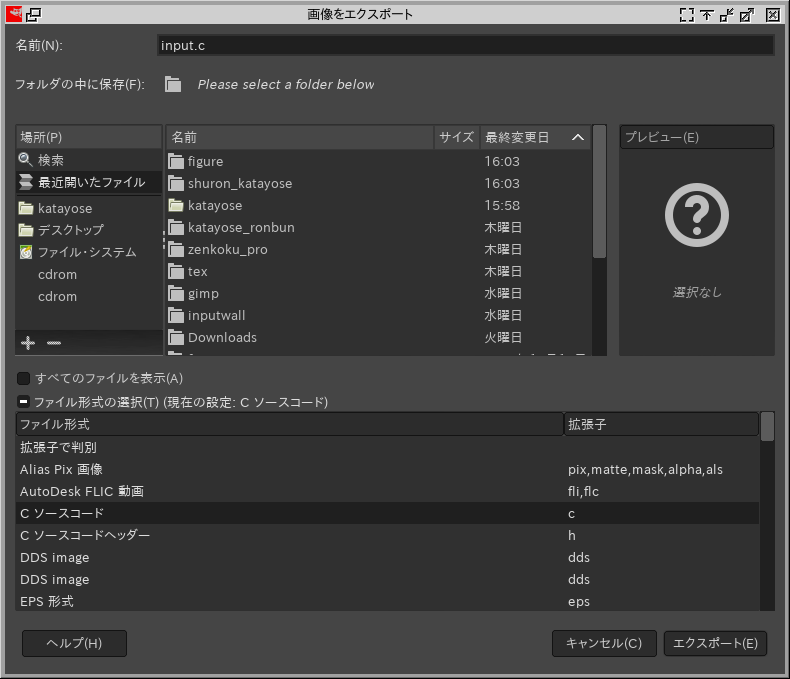
\includegraphics[width=7.5cm,clip]{figure/gimp1.png}
    \caption{GIMPの出力ファイル形式の選択}
    \label{fig:gimp1}
  \end{center}
\end{figure}


\begin{figure}[t]
  \begin{center}
    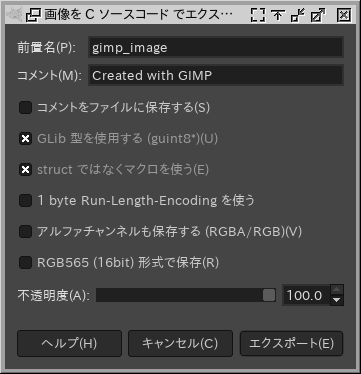
\includegraphics[width=5cm,clip]{figure/gimp2.png}
    \caption{GIMPのC言語出力画面}
    \label{fig:gimp2}
  \end{center}
\end{figure}

\section{プログラム実行時の出力フォーマット}
本プログラムを実行したときは,下記のような数字が出力される.
%
\begin{itembox}[l]{プログラム終了時の出力結果}
[格子サイズ],[前処理の時間],[解析時間],[エージェント間距離の計算回数],[壁を避ける力の計算回数]
\end{itembox}
%
また,本プログラムは解析中の様子や初期配置を出力することが可能である.
本プログラムは,画像を出力するために,gnuplotを使用しており,
使用バージョンが5.4である.
\tabref{tb:toggle_outputs}に解析中の様子をGIF形式で出力する方法や
初期配置をEPS形式で出力する方法を示す.
それぞれの出力方法を設定した場合は,プログラム終了時にtest.gifやtest.eps
のファイル名で出力される.

\begin{table}[t]
  \begin{center}
    \caption{出力の設定方法}
    \label{tb:toggle_outputs}
    \begin{tabular}{c|c}
      \hline \hline
      出力形式 & 出力方法 \\ \hline
      EPS形式  & プログラム中で「\#DEFINE EPS」と記述する.\\ \hline
      GIF形式  & プログラム中で「\#DEFINE GIF」と記述する.\\ \hline
    \end{tabular}
  \end{center}
\end{table}
%***** END ************************************************